% !TEX TS-program = xelatex
%
\documentclass{beamer}

\usetheme{Dresden}

\usepackage{fontspec}
\defaultfontfeatures{Ligatures=TeX}

\usepackage{upgreek}
\usepackage{setspace}

\usepackage{tkz-graph}
\tikzset{vertex/.style = {shape=circle,draw,minimum size=1}}
\tikzset{edge/.style = {->,> = latex'}}

\hypersetup
{
  pdftitle   = {Process Calculi for Concurrency},
  pdfauthor  = {Michael Kaltschmid \& Markus Reiter}
}

\title{Process Calculi for Concurrency}
\author{Michael Kaltschmid \& Markus Reiter}
\date{}

\begin{document}
  \maketitle

  \begin{frame}{Outline}
    \begin{itemize}
      \item $\upmu$-Calculus
      \item $\mu$-Calculus
      \item µ-Calculus
      \item mCRL2
    \end{itemize}
  \end{frame}

  \begin{frame}{Syntax}
    The set of µ-calculus formulas, $\mathcal{F}$ is the smallest set containing: \\[12pt]
    \begin{spacing}{1.2}
      $p$ and $\neg p$ for all propositions $p \in Prop$ \\
      $X$ for all variables $X \in Var$ \\
      $\phi \lor \psi$ and $\phi \land \psi$, if $\phi$, $\psi$ are formulas in $\mathcal{F}$ \\
      ($a$)$\phi$ and [$a$]$\psi$, if $a \in Act$ is an action and $\phi$ is a formual in  $\mathcal{F}$ \\
      $\mu X. \phi$ and $v X. \phi$, if $X \in Var$ is a variable and $\phi \in \mathcal{F}$ is a formula. \\
    \end{spacing}
  \end{frame}

  \begin{frame}{Diamond \& Box Modalities}
    \resizebox{\textwidth}{!}{
      \renewcommand{\arraystretch}{2}
      \begin{tabular}{l c c c c}
        &

        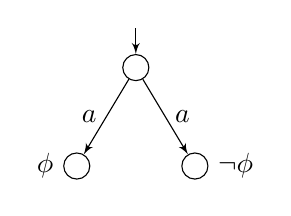
\begin{tikzpicture}
          \node[vertex] (a) at (0.75, 1.25) {};
          \node[vertex] [label=left:{$\phi$}] (b) at (0, 0) {};
          \node[vertex] [label=right:{$\neg\phi$}] (c) at (1.5, 0) {};

          \draw[edge] (.75, 1.75) to (a);
          \draw[edge] (a) to node [left] {$a$} (b);
          \draw[edge] (a) to node [right] {$a$} (c);
        \end{tikzpicture}

        &

        \begin{tikzpicture}
          \node[vertex] (a) at (0, 1.25) {};
          \node at (0, -0.175) {};

          \draw[edge] (0, 1.75) to (a);
        \end{tikzpicture}

        &

        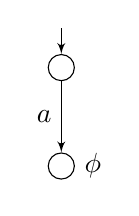
\begin{tikzpicture}
          \node[vertex] (a) at (0, 1.25) {};
          \node[vertex] [label=right:{$\phi$}] (b) at (0, 0) {};

          \draw[edge] (0, 1.75) to (a);
          \draw[edge] (a) to node [left] {$a$} (b);
        \end{tikzpicture}

        &

        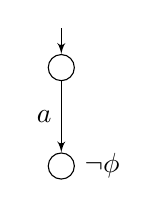
\begin{tikzpicture}
          \node[vertex] (a) at (0, 1.25) {};
          \node[vertex] [label=right:{$\neg\phi$}] (b) at (0, 0) {};

          \draw[edge] (0, 1.75) to (a);
          \draw[edge] (a) to node [left] {$a$} (b);
        \end{tikzpicture}

        \\

        $\langle{}a\rangle{}\phi$ & valid   & invalid & valid & invalid \\

        $[a]\phi$                 & invalid & valid   & valid & invalid \\
      \end{tabular}
    }
  \end{frame}
\end{document}
